\section{hklklk}

\subsection{Che cos'è il floating point}
Dato che in informatica non è possibile implementare il concetto di infinito (a differenza della matematica) non si è in grado di rappresentare tutto l'insieme dei reali; pertanto occorre, per forza di cose, approssimarlo. Il metodo che oggi è comune per il calcolo scientifico è noto come sistema \textbf{floating point} che permette una rappresentazione di ampio intervallo della retta reale con una distribuzione uniforme degli errori 


\subsection{Definizione formale}
\definizione{
    Si definisce \textbf{inseime dei numeri numeri macchina}  (floating point) con $t$ cifre significative, con base $\beta$, con $p \in [L,U]$ e con le cifre $d_i$ dove $0 \leq d_i \leq \beta -1$, $i = 1, 2, \dots$ e $d_1 \neq 0$
    \[
        \mathbb{F}(\beta, t, L, U) =  \{ 0 \} \cup \{ x \in \mathbb{R} = \text{sign}(x) \beta^{p} \sum_{i=1}^{t} d_i \beta^{-i} \}
    \]
    Usualmente $U$ è positivo e $L$ negativo
}

Questo insieme è, quindi, un'approssimazione all'intervallo preciso di numeri $[min, max] \subseteq \mathbb{R}$ che dipendono da $U$ e $L$. Se voglio rappresentare un numero maggiore/minore di questo intervallo avrò un errore chiamato \textbf{overflow/underflow}



\subsection{Gap}
con questa notazione non è impossibile scrivere ogni numero presente nella retta dei numeri Reali $\mathbb{R}$, ma tra due numeri vi è sempre una certa distanza quindi è pertanto vero che $\mathbb{F}\subseteq \mathbb{R}$. Questo concetto introduce la definizione di Gap:
\definizione{
    Chiamiamo \textbf{gap} la distanza da un numero al suo sucessivo
}
È, inoltre, vero che il gap rimane costante quando l'esponente non cambia, mentre se nell'insieme $\mathbb{F}$ il sucessivo di un numero ha un espente diverso il suo gap sarà diverso di quello del suo precedente con l'esponente uguale. Facciamo un esempio per rendere il tutto più chiaro:
\esempio{
    Sia $\beta = 2, t = 3, L = -1, U=2$ allora
    \[
        \mathbb{F}(2,3,-1,2) = \{0\}\cup\{0.100\times2^p, 0.101\times2^p, 0.110\times2^p,0.111\times2^p, p = -1, 0,1,2\}
    \]
    Questo insieme rappresenta 33 nuemri compreso lo 0:

    %! RIFARE BENE
    \begin{multicols}{4}
        \[
        \begin{array}{c}
        .100(-1) \\
        \frac{1}{4} \\
        .100(0) \\
        \frac{1}{2} \\
        .100(1) \\
        1 \\
        .100(2) \\
        2
        \end{array}
        \]
        \columnbreak
        \[
        \begin{array}{c}
        .101(-1) \\
        \frac{5}{16} \\
        .101(0) \\
        \frac{5}{8} \\
        .101(1) \\
        \frac{5}{4} \\
        .101(2) \\
        \frac{5}{2}
        \end{array}
        \]
        \columnbreak
        \[
        \begin{array}{c}
        .110(-1) \\
        \frac{6}{16} \\
        .110(0) \\
        \frac{6}{8} \\
        .110(1) \\
        \frac{6}{4} \\
        .110(2) \\
        \frac{6}{2}
        \end{array}
        \]
        \columnbreak
        \[
        \begin{array}{c}
        .111(-1) \\
        \frac{7}{16} \\
        .111(0) \\
        \frac{7}{8} \\
        .111(1) \\
        \frac{7}{4} \\
        .111(2) \\
        \frac{7}{2}
        \end{array}
        \]
    \end{multicols}
    La rappresentazione di $\mathbb{F}$ nella retta dei numeri reali è questa
    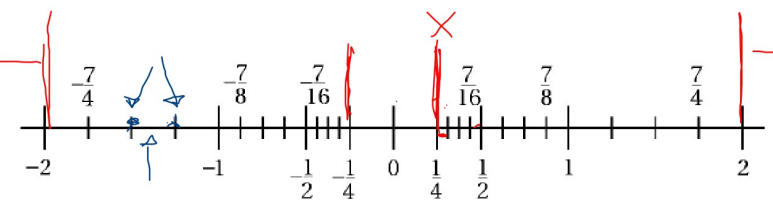
\includegraphics[width=10cm]{retta_reale.png}
}

Risulta quindi evidente l'aumento dell'ampiezza degli intervalli definiti dal valore $p$, in ognuno dai quali vengono localizzati le $t$ cifre della mantissa; ne risulta di conseguenza una diradazione delle suddvisioni verso gli estremi sinistro e destro della retta reale. \\
Il numero $t$, quindi, fissa la precisione di rappresentazione di ogni numero; infatti la retta viene suddivisa in intervalli $[\beta^p,\beta^{p+1}]$  di ampiezza crescente e in questi intervalli viene vengono rappresentati lo stesso numero $(\beta-1)\beta^{t-1}$ di valori, generando ,così, una suddivisione molto densa per valori vincini allo 0 e più rada per valori grandi in valore assoluto. Di conseguenza si ha che \textbf{maggiore è il numero $t$ di cifre della mantissa, minore sarà l'ampiezza dei intervalli e quindi migliore l'approssimazione introdotta}

\subsection{floating point nei calcolatori}
La rappresentazione più comune del sistema nei calcolatori è definita dallo Standand IEEE 745 il cui insieme è $\mathbb{F}(2,52,1023,1024)$ ed è descritta dalla formula
\[
    n = (-1)^s \cdot 2^{e-1023} \cdot (1+f)   
\]

Dove: 
\begin{itemize}
    \item \textbf{s}: è un bit che determina il segno del numero. Se $s=0$ il numero è positivo, se $s=1$ il numero è negativo.
    \item \textbf{e}: è l'esponente del numero due, ed è un intero di 11 bit tale che $e \in [0,2047]$.
    \item \textbf{f}: il valore detto \textbf{mantissa} è una serie di 52 bit che rappresenta la parte frazionaria del numero, nel nostro caso $f \in [0,1]$.
    \item \textbf{1023}: è detto \textbf{bias} ed è usato per codificare esponenti negativi e positivi.
\end{itemize}
In memoria si traduce in un array contentente questi bit:
\begin{center}
    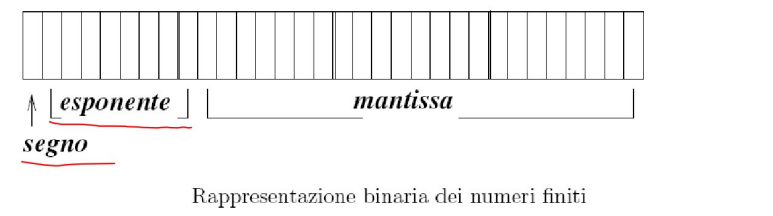
\includegraphics[width=7cm]{floating_point_in_memoria.png}
\end{center}

\esempio{
    Per trovare la codifica del numero in floating point 1 10000000010 1000000000000000000000000000000000000000000000000000 in base 10 occorre:
    \begin{enumerate}
        \item Trovare l'esponente decimale, che è $1 \times 2^{10} + 1 \times 10^1 - 1023 = 3$.
        \item Trovare la parte frazionaria, che è $1 \times \frac{1}{2^1} = 0,5$.
    \end{enumerate}

    Quindi $n = (-1)^1 \times 2^3 \times (1+0,5) = -12,0$.
}

\subsection{troncamento}

Sia l'insieme $\mathbb{F}(\beta, t, L, U) =\{ \{\emptyset\} \cup n = \pm \beta^p \cdot d_0 d_1 \dots d_t  \} $ con $-L \leq p \leq U$ l'insieme dei numeri floating point caratterizzati dai valori $\beta, t, L, U$

Inoltre sia $x \in \mathbb{R}$ dove $x = \pm \beta^p \cdot d_0 d_1 \dots d_t, d_{t+1}, \dots$ con $L\leq p \leq U$, nel caso in cui $x \notin \mathbb{F} $ rappresento $x$ con un elemento di $\mathbb{F} $ che indico con $fl(x) = \pm \beta^p \cdot d_0 d_1 \dots d_t$. Questa operzione si chiama \textbf{troncamento}

\subsection{Errore relativo di arrotondamento}
Il sistema floating point dato che è un'approssimazione è ovvio che la precisione di rappresentazione che offre non è perfetta, in quanto i numeri infiniti (come il $\pi$) vengono delineati con una serie finita di numeri finiti. La differenza tra la sua approssimazione e il suo valore reale è detta \textbf{errore di arrotondamento}  
\subsubsection{definizione}
klkjlkjkljlkj
\definizione{
    Sia $x\in \mathbb{R}$ un numero reale e sia $fl(x)$ (dove $fl()$ è la funzione arrotondamento) il numero $x$ arrotondato, allora l'errore realtivo di arrotondamento è definito dalla seguente formula:
    \[
        \frac{|fl(x)-x|}{|x|} \leq \frac{1}{2}\beta^{1-t}
    \]
}
 La quantità $esp=\frac{1}{2}\beta^{1-t}$ è detta  \textbf{precisione macchina} nel sistema floating point, ed è il più piccolo numero macchina positivo tale che: 
 \[
    fl(1+esp)>1
 \]

\subsection{artimetica floating point}
Il calcolatore esegue operazioni solo con numeri rappresentabili da calcolatore stesso, quindi in questo caso dai numeri scritti in forma floating ponti (per i nuemri reali), il punto è che \red{le usuali operazioni aritmetiche non sono chiuse nell'insieme $\mathbb{F}$}, quindi presi 2 numeri dall'insieme $\mathbb{F}$ e computati tramite operazioni aritmetiche, il risultato di tale computazione potrebbe appartenere nell'insieme $\mathbb{R}$. Pertanto \red{i risultati delle varie computazioni dovranno essere sempre arrotondati ad un numero che stia in $\mathbb{F}$}
\subsubsection{operazione floating point} 
L'operazione floating point (o di macchina) è definita
\definizione{
    \[
        \odot :\mathbb{R}\times\mathbb{R}\rightarrow\mathbb{R}
    \]
}
Ogni operazione provoca un piccolo errore detto \textbf{errore di arrotondamento}:
\[
    |\frac{(x\odot y)-(x\cdot y)}{x\cdot y}|<eps
\]

l'operazione floating point nei calcolatori viene strutturata in due fase:
\begin{enumerate}
    \item \textbf{Eseguo l'operazione esatta}: (es. $z=x+y$) dove viene fatta utilizzando più bit utilizzati di quelli utilizzati per memorizzare il risultato, non è accessibile all'utente ma viene memorizzato in un registro interno alla cpu
    \item \textbf{Trocamento del risultato}: (es. $x\oplus y = fl(z)$), dove una volta che il calcolo è stato fatto in precisione estesa il risultato viene arrotondato alla precisione del risultato
\end{enumerate}
\esempio{
    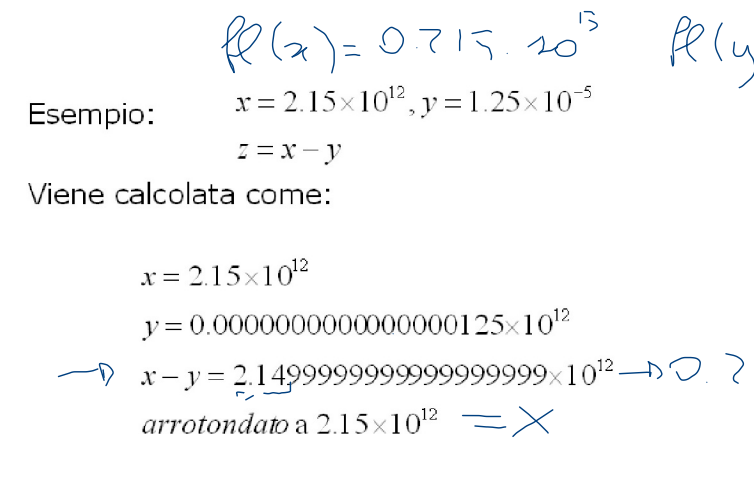
\includegraphics[width=10cm]{arrotondamento_esempio.png}
}
